\chapter{Literature Review}\label{chapter:background}

\textit{Give a background on basketball, sports predictions in general, sports predictions on basketball and theoretical concepts used in the report.}

\section{Analytics in Sports}


\subsection{Baseball}
Baseball can be seen as the beginning for sports analytics \citep{moneyball}.  The Oakland Athletics could not compete financially with the bigger teams of Major League Baseball, thus general manager Billy Beane used 
\subsection{American Football}

\subsection{English Football}
Dixon and Coles developed a model that uses full-time scores to predict the probabilities of a future match \citep{dixon_coles}.

Dixon and Robinson extended the model created by Dixon and Coles by modelling goal times \citep{dixon_robinson}.

\section{Prediction in the National Basketball Association}
\textit{Talk about the history of data science in the NBA}

\textit{Talk about nba advanced stats.}

% Streak Shooting
There is a belief among basketball players and fans that a player will be more likely to score following a previous successful shot rather than a miss.  A survey was conducted of NBA fans, where 91\% of fans believed that a player has a better chance of scoring after having just made his last two or three shots than after missing the same number \citep{nba_hot_hand}.  Shooting records from the Philadelphia 76ers and it's opponents were analysed from the 1980-81 season.   The analysis provided no evidence towards streak shooting.  Free throw data from the Boston Celtics during the 1980-81 and 1981-82 seasons were also analysed to remove the presence of shot selection and defensive pressure.  Again, no evidence was found the second free throw was affected by the first.  Finally, an experiment with the players from Cornell University as an alternative way to eliminate shot selection and defensive pressure \citep{nba_hot_hand}.  The conclusion of the Cornell experiment is that previous shots 
influenced the players' predictions, but not their performance.  

% Team Cohesion
Team cohesion is an important factor to consider as research studies have shown that highly cohesive teams are likely to be highly successful teams \citep{team_cohesion}.  Research was done to evaluate team cohesion and performance in the basketball league in Kenya \citep{basketball_team_cohesion}.  The participants were athletes who had at least two years experience in the league.  Six players were randomly selected from each team in the league.  The results show that 96\% of players believed they played and won as a team while 76\% believed they lost as a team.  An analysis of variance (ANOVA) test was conducted, which shows that teams with a higher cohesion between players won more frequently than teams with low cohesion.  There was a significant relationship shown between team size and team cohesion.  In the NBA, there is a maximum amount of players allowed per team, so this may not affect this league on the same level.  While the studies show that team cohesion leads to success, it would be difficult to translate that into a statistical model.

% NBA Defense
Most of basketball advanced metrics have been developed for offence as offensive performance is more easily measured due to the number of statistics pertaining to scoring.  Although there are statistics such as steals and blocks that provide some insight into a player's defensive performance, they do not show the full story.  Thus, there have been attempts to model defensive performance by introducing new defensive metrics utilising the the emerging forms of player tracking information \citep{nba_defense}.  The model created by Franks et. al. \citep{nba_defense} begins by estimating defensive matchups for every moment in a basketball game.  The matchups allows us to see which defenders are responsible for which attacking player at different stages of an offensive possession, including when points are scored.  Table \ref{table:defensive_metrics} shows the metrics introduced.  These metrics make it easier to see who are the best and worst defenders in the league and could greatly improve the performance of a statistical model.

\begin{table}[ht]
\centering
\begin{tabular}{|l|l|}
\hline
\textbf{Defensive Metric} & \textbf{Description} \\ \hline
Volume Score & \begin{tabular}[c]{@{}l@{}}The total number of shot attempts a defender faces.\end{tabular}\\ \hline
Disruption Score & \begin{tabular}[c]{@{}l@{}}A defender's ability to reduce the \\  effectiveness of his opponent's shots.\end{tabular}\\ \hline
Defensive Shot Chart & \begin{tabular}[c]{@{}l@{}}Similar to an offensive shot chart, but\\ for defensive shots against.\end{tabular}\\ \hline
Shots Against & \begin{tabular}[c]{@{}l@{}}Weighted average of shots attempted\\ against the defender per 100 possessions.\end{tabular}\\ \hline
Counterpoints & \begin{tabular}[c]{@{}l@{}}Weighted average of points scored\\ against the defender per 100 possessions.\end{tabular}\\ \hline

\end{tabular}
\caption{Defensive Player Metrics}
\label{table:defensive_metrics}
\end{table}

% Shot Selection
Shot selection is a very important part of offence in basketball.  \ldots can capture the correlation between a player's skill and shooting habits.
Shot selection \cite{nba_spatial_analysis}.

% NBA Taxonomy
Again, player tracking data was analysed to dissect basketball plays using acceleration \citep{nba_taxonomy}.  Further research in this subject could lead to classifying team philosophies and using that information when predicting opposing play styles (For example a high tempo offence against a very lax defence)

% Fuzzy Classification
A fuzzy classification system has been developed to predict the winner of a game from the Asociaci\'on de Clubes de Baloncesto, the professional basketball league in Spain \citep{nba_fuzzy_prediction}.  Eight different feature selection algorithms were used and the most consistent features selected were the average number of assists by the first team, the teams' evaluations and the average points scored by each team.  Eleven different fuzzy algorithms were used, with accuracies ranging from 63.5\% to 71.5\%.

\section{Mathematical Concepts}
The following section will describe the mathematical concepts used in the modelling done in this report.

\subsection{Poisson Distribution}
The Poisson distribution is defined by the formula \cite{poisson}

\begin{equation}
p_x(\lambda) = \frac{e^{-\lambda}\lambda^x}{x!}
\end{equation}

Figure \ref{fig:poisson} shows the probability mass function for the Poisson distribution with various $\lambda$.  The $y$ axis is the probability of $k$ occurring given the mean $\lambda$.  \textit{Cite This ->} The function is only defined at integer values of $k$.

\begin{figure}[!htb]
	\centering
	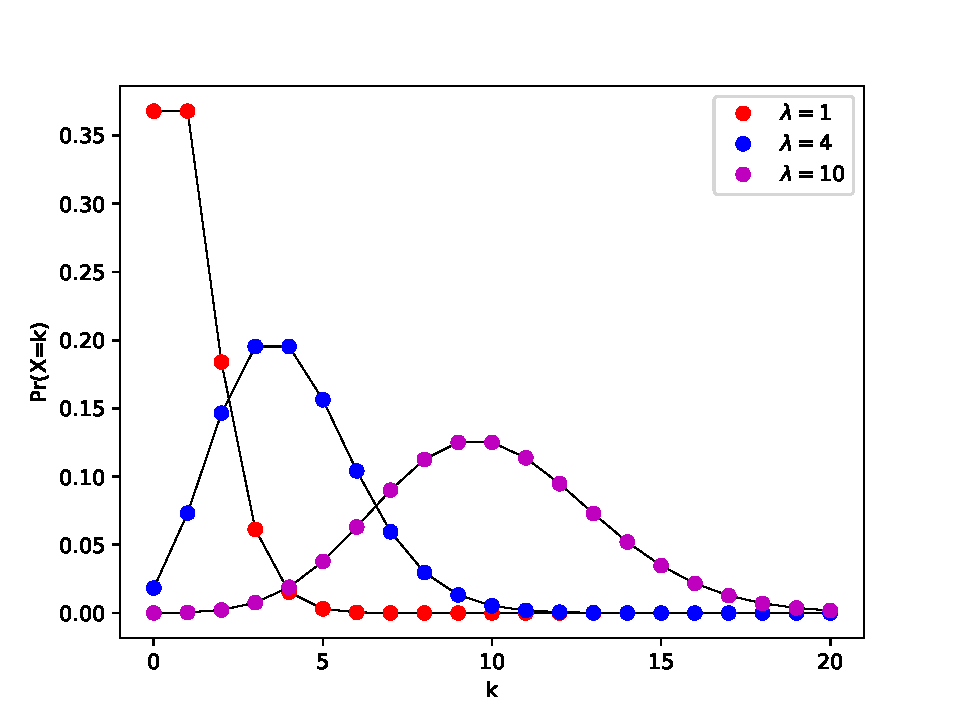
\includegraphics[width=0.75\textwidth]{{Figures/poisson_dist.pdf}}
	\captionof{figure}{Probability mass function of the Poisson Distribution}
	\label{fig:poisson}
\end{figure}

\subsection{Beta Distribution}

The Beta distribution is a probability distribution defined on the interval $[0, 1]$